% Quality assurance for ProfiSnort
\documentclass[listof=totoc,a4paper]{scrreprt}

\usepackage[german]{babel}
\usepackage[utf8]{inputenc}
\usepackage[T1]{fontenc}
\usepackage{ae}
\usepackage[bookmarks,bookmarksnumbered]{hyperref}
\usepackage{csquotes}
\usepackage{longtable}
\usepackage{enumitem, hyperref}
\usepackage{graphicx}

\usepackage{float}
\usepackage{verbatim}
\usepackage{rotating}
\usepackage{placeins}

\usepackage[ampersand]{easylist}
\usepackage{xcolor}

\usepackage[toc,acronym]{glossaries}
\makeglossaries

\setuptoc{toc}{totoc}
\setcounter{tocdepth}{2}

\usepackage{xparse}
\DeclareDocumentCommand{\newdualentry}{ O{} O{} m m m m } {
  \newglossaryentry{gls-#3}{name={#5},text={#5\glsadd{#3}},
    description={#6},#1
  }
  \makeglossaries
  \newacronym[see={[Glossary:]{gls-#3}},#2]{#3}{#4}{#5\glsadd{gls-#3}}
}

\renewcommand*{\glstextformat}[1]{\textcolor{black}{#1}}

\hypersetup{
	backref,
    colorlinks,
    linkcolor=[RGB]{0,153,84},
    citecolor={blue!40!black},
    urlcolor={blue!70!black},
    linktocpage=true
}

\makeatletter
\def\namedlabel#1#2{\begingroup
    #2%
    \def\@currentlabel{#2}%
    \phantomsection\label{#1}\endgroup
}
\makeatother

\newcounter{savepage}

\newcommand{\sppname}{spp\_profinet}
\newcommand{\programname}{TruffleHog}

\loadglsentries{../global_tex_files/glossary}

\setlength{\parindent}{0em}

\begin{document}

\title{\programname \ \& \sppname \ -- Testbericht}
\author{
    Brendl, Julian
    \texttt{julian.brendl@student.kit.edu}
    \and
    Diez, Maximilian
    \texttt{maximilian.diez@student.kit.edu}
    \and
    Giraud, Mark
    \texttt{mark.giraud@student.kit.edu}
    \and
    Hermes, Jan
    \texttt{jan.hermes@student.kit.edu}
    \and
    Höhler, Dimitri
    \texttt{dimitri.hoehler@student.kit.edu}
    \and
    Kiechle, Valentin
    \texttt{valentin.kiechle@student.kit.edu}
}

\titlehead{\includegraphics[width=150pt]{images/title.png}}

\maketitle

\pagenumbering{Roman}
\setcounter{page}{2}

\newpage
\tableofcontents
\newpage
\listoffigures

%\printglossary[title=Abkürzungsverzeichnis,toctitle=Abkürzungsverzeichnis,type=acronym]

\clearpage
\setcounter{savepage}{\arabic{page}}
\pagenumbering{arabic}
\setcounter{page}{\thesavepage}

\chapter{Einleitung}

Dieses Dokument dient der Qualitätssicherung der TruffleHog Software sowie einer kurzen Beschreibung der Designänderungen, die während der Implementierung vorgenommen wurden.
Zum einen wird beschrieben, welche Maßnahmen zum Erreichen der Korrektheit der Software ergriffen wurden. Das schliesst sowohl JUnit Tests und deren Line Coverage, als auch im Pflichenheft definierte Testzenarien ein, welche das Nutzerverhalten simulieren sollen. Des Weiteren wird erläutert welche größeren Probleme bei der Implementierung und beim Testen auftraten, und wie diese Bugs behoben wurden.
% Functional specification for ProfiSnort
\documentclass[listof=totoc,a4paper]{scrreprt}

\usepackage[german]{babel}
\usepackage[utf8]{inputenc}
\usepackage[T1]{fontenc}
\usepackage{ae}
\usepackage[bookmarks,bookmarksnumbered]{hyperref}
\usepackage{csquotes}
\usepackage{longtable}
\usepackage{enumitem, hyperref}
\usepackage{graphicx}

\usepackage{float}
\usepackage{verbatim}

\usepackage[ampersand]{easylist}
\usepackage{xcolor}

\usepackage[toc,acronym]{glossaries}
\makeglossaries

\setuptoc{toc}{totoc}

\usepackage{xparse}
\DeclareDocumentCommand{\newdualentry}{ O{} O{} m m m m } {
  \newglossaryentry{gls-#3}{name={#5},text={#5\glsadd{#3}},
    description={#6},#1
  }
  \makeglossaries
  \newacronym[see={[Glossary:]{gls-#3}},#2]{#3}{#4}{#5\glsadd{gls-#3}}
}

\renewcommand*{\glstextformat}[1]{\textcolor{black}{#1}}

\hypersetup{
	backref,
    colorlinks,
    linkcolor=[RGB]{0,153,84},
    citecolor={blue!40!black},
    urlcolor={blue!70!black},
    linktocpage=true
}

\makeatletter
\def\namedlabel#1#2{\begingroup
    #2%
    \def\@currentlabel{#2}%
    \phantomsection\label{#1}\endgroup
}
\makeatother

\newcounter{savepage}

\newcommand{\sppname}{spp\_profinet}
\newcommand{\programname}{TruffleHog}


\loadglsentries{../../global_tex_files/glossary}


\begin{document}

\title{\programname \ \& \sppname \ -- Entwurf}
\author{
    Brendl, Julian
    \texttt{julian.brendl@student.kit.edu}
    \and
    Diez, Maximilian
    \texttt{maximilian.diez@student.kit.edu}
    \and
    Giraud, Mark
    \texttt{mark.giraud@student.kit.edu}
    \and
    Hermes, Jan
    \texttt{jan.hermes@student.kit.edu}
    \and
    Höhler, Dimitri
    \texttt{dimitri.hoehler@student.kit.edu}
    \and
    Kiechle, Valentin
    \texttt{valentin.kiechle@student.kit.edu}
}

\titlehead{\includegraphics[width=150pt]{images/title.png}}

\maketitle

\pagenumbering{Roman}
\setcounter{page}{2}

\newpage
\tableofcontents
\newpage
\listoffigures

\printglossary[title=Abkürzungsverzeichnis,toctitle=Abkürzungsverzeichnis,type=acronym]

\clearpage
\setcounter{savepage}{\arabic{page}}
\pagenumbering{arabic}
\setcounter{page}{\thesavepage}

\chapter{Einleitung} 
Dieses Dokument dient der genaueren Beschreibung und Dokumentation des Entwurfs zum Visualisierungstool Trufflehog, dessen Hauptaufgabe die Darstellung des Netzwerkverkehrs eines ProfiNet-Systems ist. Des Weiteren wird der im IDS Snort eingebaute Präprozessor \sppname und die genaue Funktionsweise der Inter-Prozess-Kommunikation (im Folgenden IPC) zu Trufflehog genau erläutert.

Das Design von Trufflehog baut auf dem klassischen Model-View-Controller (im Folgenden MVC) auf und erweitert diesen Entwurf zu einem Model-View-Presenter mit zusätzlicher Funktionalität.

//hier MVC von Präsentation und ähnliches Bild zum aktuellen Entwurf einfügen//


\chapter{Architektur und Musterbeschreibung}
Im Groben gehalten funktioniert der Daten- und Befehlsfluss im Trufflehog-Entwurf wie im klassischen MVC, der Presenter aktiviert Services, welche das Model basierend auf dem empfangenen Netzwerkverkehr verändert und das View aktualisiert sich am Model. Da viele Threads im Programm parallel durchlaufen aber dennoch kommunizieren müssen, verlassen wir uns an einigen Stellen auf das \gls{observerpattern} mit einer Multi-Thread kompatiblen Datenstruktur.\newline
\newline


\section{\textbf{commands-Package:}}


Die Kernfunktionalität innerhalb des Programms stellt das \textbf{commands-Package}. Darin befinden sich sowohl die Hierarchie, vorhandene Datenstruktur als auch jede mögliche Command-Klasse und deren Interface. Vom Prinzip her vergleichbar mit Runnables.\newline

\begin{figure}[H]
  \centering
  \includegraphics[width=\textwidth]{../diagramimages/commands.png}
  \caption{\textbf{commands-Package}}
\end{figure}

Es gibt 2 Hauptarten von Commands, UserCommands für die Verwaltung der Benutzeroberflächenbefehle, und TruffleCommands für die Methodenaufrufe im Model-Graph, also die Hauptarbeit am Model. Die Commands machen außerdem den Hauptteil der Log-Datein und damit der Video-Funktion aus. Mehr dazu im service-Unterpackage datalogging.

    \subsection*{\textbf{commandQueue}}
    Die besagte Datenstruktur, welche beispielsweise der executor besitzt. Es sind ggf. mehrere tatsächliche Queues vorhanden, was einen Manager verlangt um nach dem Round-Robin-Prinzip faire Verteilung zu ermöglichen.


\section{\textbf{service-Package:}}


In unserem Entwurf haben wir uns außerdem dazu entschieden einzelne durchlaufende Arbeitsschritte in das \textbf{Service-Package} auszulagern.\newline

\begin{figure}[H]
  \centering
  \includegraphics[width=\textwidth]{../diagramimages/service.png}
  \caption{\textbf{service-Package}}
  \medskip
\end{figure}

    \subsection*{\textbf{truffleprocessor}}
    Der \textbf{truffleprocessor} ist die Empfangsstelle für die von uns in der \gls{ipc} benutzen Truffles. Außerdem erzeugt er die später verwendeten Commands und benachrichtigt als \gls{notifier}.
    
    \subsection*{\textbf{datalogging}}
    Das \textbf{datalogging} kümmert sich um die gesamte gewünschte Speicherung/Loggen und, falls implementiert, die Verfügbarkeit der Video-Daten. Es speichert sowohl regelmäßige Snapshots des gesamten Graphen, als auch einzelne Commands für eine Schrittweise Rückverfolgung des Ablaufes.
    
    \subsection*{\textbf{executor}}
    Der \textbf{executor} ist das Unterpackage, in welchem die Anwendung bzw. Ausführung der Commands stattfindet. Er ist ein \gls{listener} für Commands von sowohl dem view-Package als auch dem truffleprocessor.


\section{\textbf{presenter-Package:}}


Der \textbf{presenter} ist für den Aufbau von \gls{programname}, also das Initialisieren, Instanziieren und Referenzieren aller Programmelemente zuständig.

\begin{figure}[H]
  \centering
  \includegraphics[width=\textwidth]{../diagramimages/presenter.png}
  \caption{\textbf{presenter}}
\end{figure}

Er ist der erste Thread und erzeugt alle weiteren, zum Beispiel einen für jeden Service. Außerdem liest er aus einer Settings-Datei und stellt das Programm ein.
Das heisst er initialisiert bestimmte Attribute entsprechend. Danach erschöpft sich die Nützlichkeit des \textbf{presenter} bis zu einem neuen Programmstart.


\section{\textbf{util-Package:}}


Unsere Variante des \gls{observerpattern}s.

\begin{figure}[H]
  \centering
  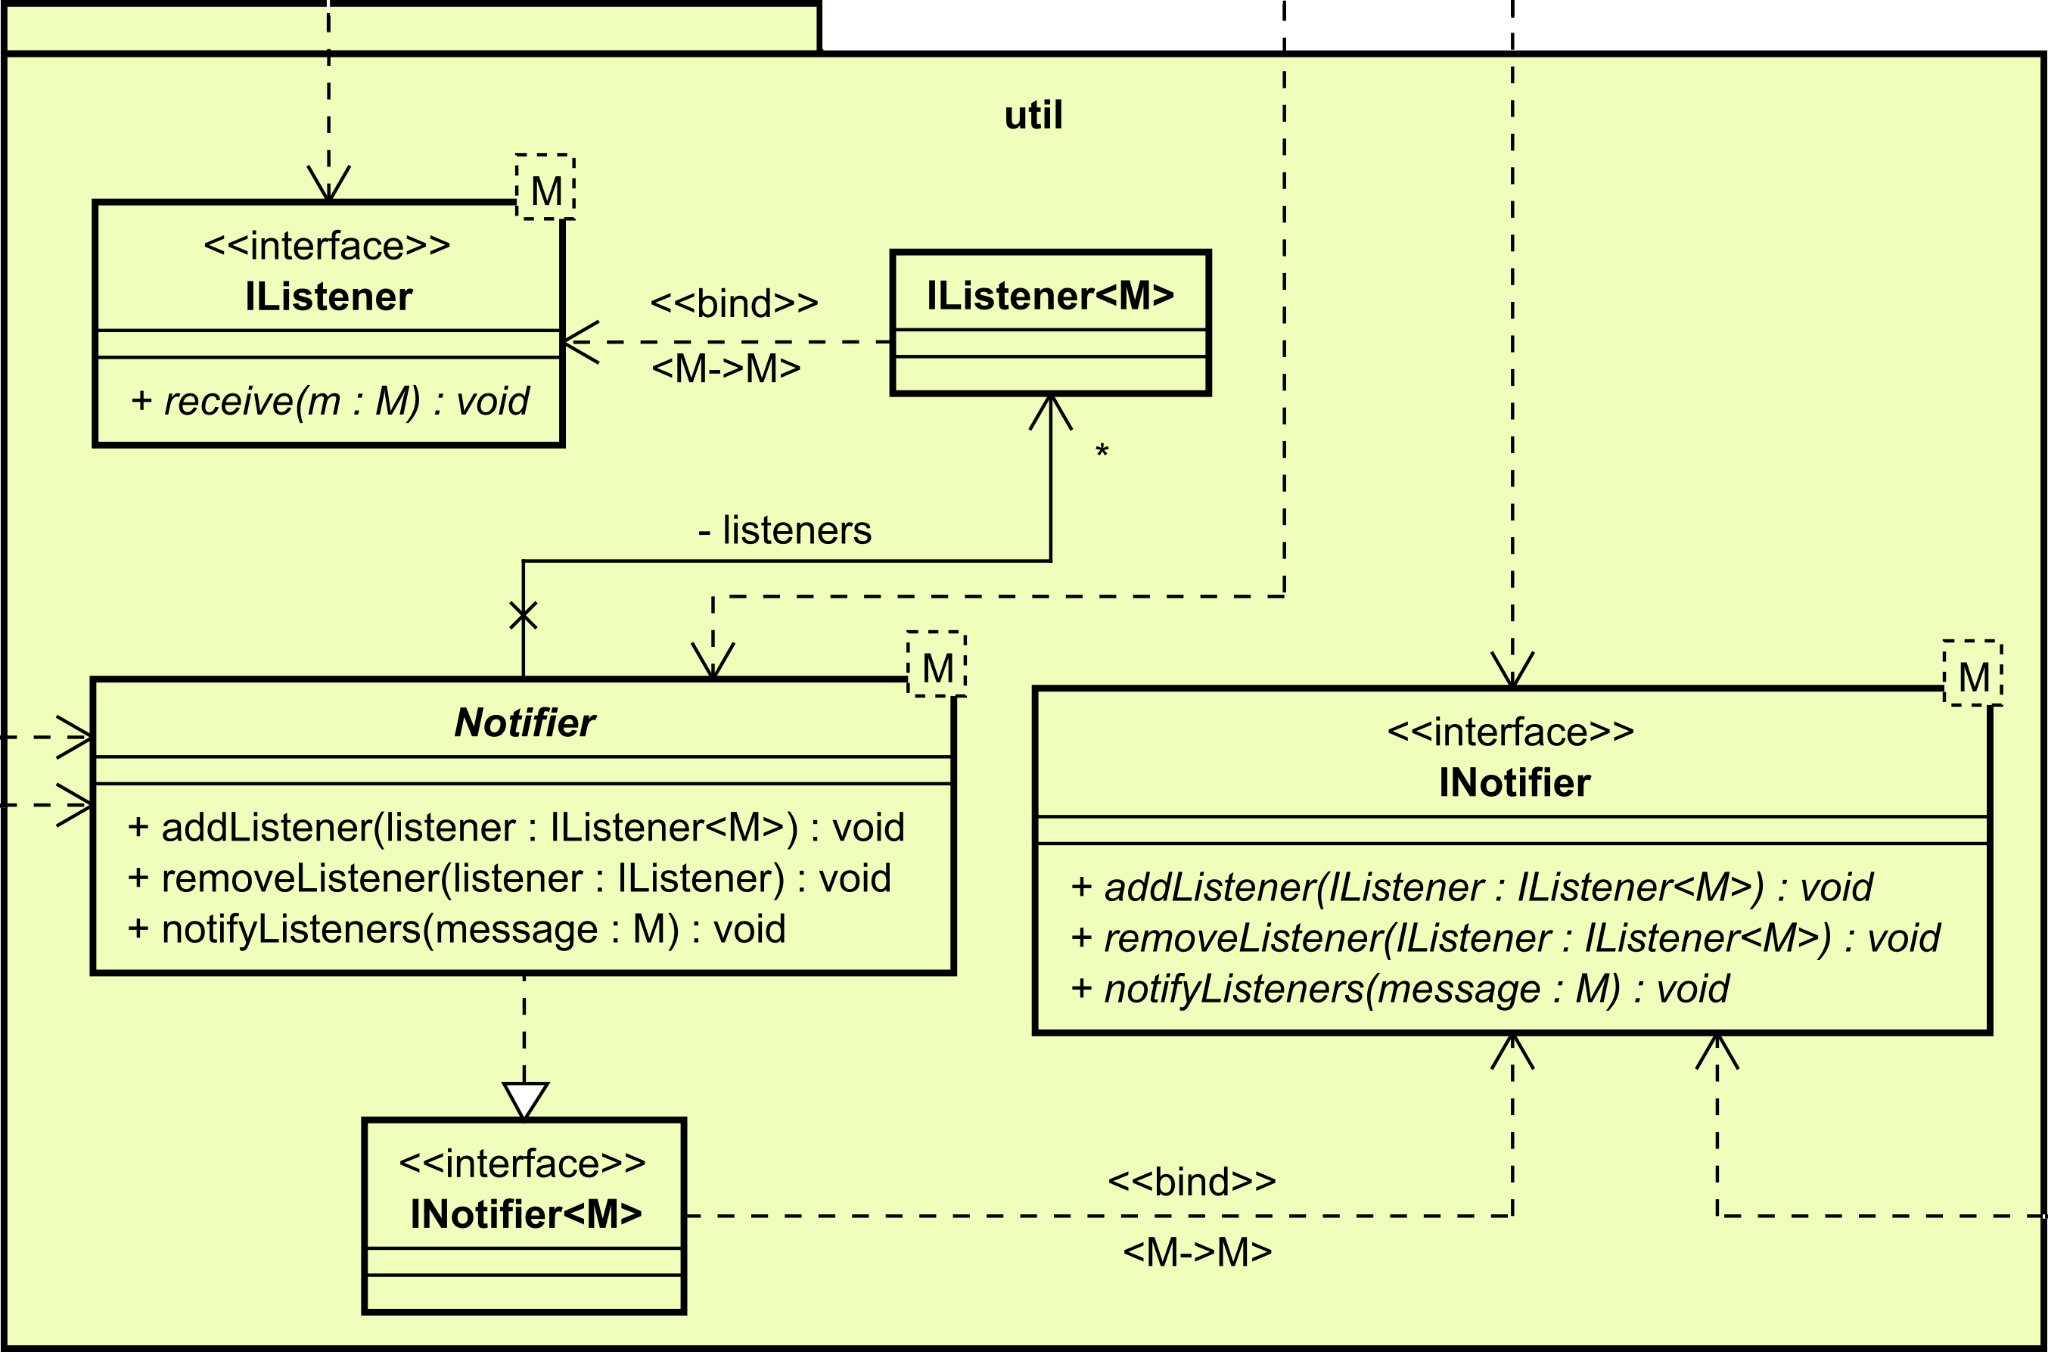
\includegraphics[width=\textwidth]{../diagramimages/util.png}
  \caption{\textbf{util-Package}}
\end{figure}

Da wir sowohl Interfaces als auch Klassen bzw. abstrakte Klassen als \gls{notifier} haben, kommen wir nicht um eine Modifizierung des klassischen \gls{observerpattern} herum. Nun haben wir die Möglichkeit sowohl ein \gls{notifier}-Interface zu erweitern als auch eine abstrakte \gls{notifier}-Klasse zu beerben. Der \gls{listener} funktioniert genau wie ein Observer.


\section{\textbf{model-Package:}}


Die Hauptdatenstruktur von \gls{programname}: das \textbf{model-Package}.

\begin{figure}[H]
  \centering
  \includegraphics[width=\textwidth]{../diagramimages/model.png}
  \caption{\textbf{model-Package}}
\end{figure}

    \subsection*{\textbf{graph}}
    
    \subsection*{\textbf{filter}}
    
    \subsection*{\textbf{settingsdata}}
    
    \subsection*{\textbf{graphlog}}


\section{\textbf{view-Package:}}


\section{\textbf{interactors-Package:}}


\chapter{Klassendokumentation}

\section{Service}

\subsection{TruffleReceiver}

\begin{figure}[h!]
    \centering
    \includegraphics[width=\textwidth]{../diagramimages/TruffleReceiver.png}
    \caption[Klasse TruffleReceiver]{Klasse TruffleReceiver}
    \medskip
    Diese Klasse empfängt ganz tolle Truffles und so ein zeug bla bla.
\end{figure}

\subsubsection*{Attribute}

\begin{easylist}[itemize]

    & Attribut 1

    & Attribut 2

\end{easylist}

\subsubsection*{Methoden}

\begin{easylist}[itemize]

    & Methode 1

    & Methode 2

\end{easylist} 

\chapter{Sequenzdiagramme}

\begin{figure}[H]
  \centering
  \includegraphics[width=\textwidth]{../diagramimages/spp-profinet-package-dissection.png}
  \caption[Sequenzdiagramm \sppname package dissection]{Sequenzdiagramm \sppname package dissection}
\end{figure}

In dieser Sequenz werden zwei zentrale Aufrufe von \gls{snort} im \gls{praeprozessor} \sppname dargestellt. Zum einen im oberen Teil die Initialisierung des \gls{praeprozessor}s durch einen Init-Aufruf, sowie der \gls{praeprozessor}-interne Aufbau des DecoderRegisters. Dieser Registrierungsvorgang wurde im Diagramm aus Platzgründen eingespaart. Darin wird jeder als C-Datei vorhandene Decoder instanziiert und bei der DecoderRegisterList registriert. Dieser Vorgang legt die Grundlage für den Decoder-Baum-Ablauf, welcher exemplarisch als zweiter unterer Teil des Sequenzdiagramms 

\chapter{Ressourcen}
\section{Dateien und Strukturen}
Im Folgenden ist das Datenhaltungsverzeichnis von \gls{programname} visualisiert. Alle persistenten, das heißt einen Neustart des Programms überdauernden Daten sind in Dateien in Unterordnern des Ordners \texttt{data} gespeichert.  
\begin{figure}[H]
  \centering
\begin{verbatim}
.
`-- data
    |-- config
    |   |-- filtermenu_en.properties
    |   |-- graphwindow_en.properties
    |   |-- logwindow_en.properties
    |   |-- notificationview_en.properties
    |   |-- settingsmenu_en.properties
    |   `-- statistics_en.properties
    |-- log
    |   `-- trufflehog.log
    |-- replay_log
    |   |-- graph_TIMESTAMP2.trufflesnapshot
    |   `-- graph_TIMESTAMP.trufflesnapshot
    `-- truffle_data_log
        |-- nodeA.xml
        `-- nodeB.xml
\end{verbatim}
  \caption[Ordner- und Dateiestruktur von \gls{programname}]{Ordner- und Dateiestruktur von \gls{programname}}
\end{figure}



\input{chapters/classindex}

\appendix

\printglossary[title=Glossar,toctitle=Glossar]

\end{document}

\chapter{Testergebnisse}

Diese Sektion beschreibt den Aufbau der Tests für \gls{programname} und \gls{sppname} sowie die dafür genutzten Testbibliotheken. Zusätzlich werden zusammenfassend Ergebnisse und Erklärungen zur Testüberdeckung bereitgestellt.

\section{\programname}

Für die Unit Tests von \gls{programname} wurde die Testbibliothek JUnit in der Version 4.11 in Kombination mit dem Mocking Framework Mockito in der Version 1.8.4 verwendet.

Um korrekte und ausführliche Tests bei der Entwicklung zu fördern, wurde im Entwicklungs-Repository von TruffleHog auf github.com eine Kontrollinstanz namens Travis-CI (https://travis-ci.org/) verwendet. Aufgabe dieses Tools ist das ausführen und validieren aller Tests von TruffleHog bei jedem Commit in den Master Entwicklungsbranch. Auf diese Weise wurden fehlerhafte Commits aus dem Master Branch fern gehalten und die Entwicklung des Projekt nicht gestört.

\subsection{Command Package}

Die zentrale Ausführungslogik von TruffleHog war im besonderen Fokus der Tests. Auf das Testen von trivialen Methoden wie Getter/Setter wurde verzichtet. Daher beträgt die Line Coverage im Command Package  70\%. Es wurden alle Klassen auf Funktionalität in den wenigen möglichen Anwendungsfällen geprüft.

\subsection{Interaction Package}
Ein Paket ohne Funktionalität. Eine Ansammlung von Enums, welche für die Überleitung von Benutzerinteraktion zu Commands gebraucht werden. Das aktive Testen entfällt daher. Durch Aufrufe anderer Tests kommt das Paket jedoch auf 81\% Line Coverage.

\subsection{Model Package}
Das größe Paket mit etwa 2000 Zeilen Programmcode. Eine hohe Coverage lies sich nicht erreichen, da die bereits getestete Graphbibliothek Jung tief eingebunden wurde und diese natürlich nicht zu Coverage beiträgt. Wieder wurden einfache Setter/Getter vom Testen ausgeschlossen, von denen es realtiv viele in der Graphstruktur gibt. Die Line Coverage beträgt 39\%.

\subsection{Presenter Package}

Da dieses Paket lediglich für den initialen Aufbau der internen Strukturen und Abhängigkeiten zuständig ist, wird die gesamte Funktionalität genau einmal pro Programmstart genutzt. Es gibt nur einfache Tests, da der Presenter nur in einem Kontext verwendet werden kann. Fehler in diesem Programm Paket würden ebenfalls sehr schnell in den Testszenarien auffallen, da die gesamte Benutzeroberfläche hierdurch aufgebaut wird. Line Coverage beträgt 77\%.

\subsection{Service Package}

Die Hauptarbeitsroutinen von TruffleHog werden im Gegensatz zum Presenter zwar regelmäßig aufgerufen, haben aber einen sehr spezifischen Einsatzbereich und wenig Variationsmöglichkeit der Parameter. Der Testfokus lag daher auf der korrekten Ausführung von mehreren Befehlen und die Einhaltung der Command Reihenfolge anstatt unmögliche Eingaben zu testen. Die relativ niedrige Line Coverage von 38\% lässt sich durch zwei Dinge begründen. Zum einen wird das ReplayLogging Service im fertigen Programm nicht verwendet und ist daher ungetestet. Zum anderen wurden für die Inter-Prozess-Kommunikationsschnittstelle eine Vielzahl von eigenen Exceptions definiert um das Debugging zu erleichtern. Diese Exceptions unterscheiden sich fast ausschliesslich im Namen, um den Fehler schnell zu finden, aber rufen getestete Methoden der Superklassen auf, daher sind diese Exceptions nicht Teil der Line Coverage.

\subsection{Util Package}

Ein Hilfspaket, hauptsächlich für die Umsetzung von Designpatterns und PropertyBindings gedacht, bietet selbst nur begrenzte aber generische Funktionalität. Methoden der PropertyBindings, die ausschliesslich Methoden der Java Superklassen verwenden sind von den Tests ausgeschlossen. Line Coverage beträgt 47\%.

\subsection{View Package}

Der Hauptbenutzeroberfläche von TruffleHog liegt JavaFX zugrunde. Alle nichttrivialen Tests werden von den Testszenarien abgedeckt. Daher beträgt die Line Coverage 31\%.

\subsection{Viewmodel Package}

Ein aufgearbeitetes Zwischenmodel, das der View direkt aufgearbeitete Daten zum Ablesen bereitstellt. Dies betrifft vor allem statistische Informationen. Coverage beträgt 66\%.

\section{\sppname}
Für \sppname wurde ein eigens entwickeltes Testing Framework entwickelt (Basierend auf Programmcode im Buch "Learn C the hard way" von Zed A. Shaw). Mit Hilfe von Makros und Bash Scripts ist dadurch eine komplett automatisiertes Testen der einzelnen Quelldateien und definierten Methoden möglich. Es wurden keinerlei Analysemöglichkeiten für die Testabdeckung implementiert, daher fehlt diese Information im Testbericht zu \gls{sppname}.

Beim Testen der einzelnen Dissektoren wurde außerdem das Programm Scapy und der darauf basierende, frei verfügbare Packetfuzzer ProFuzz (https://github.com/HSASec/ProFuzz) verwendet, um die Integrität des Dekodierungsprozesses sicherzustellen.

	\subsection{Dissect Package}
	In diesem Paket wurde lediglich die Datenstruktur DissectorRegister getestet. Bei "Dissector"{} handelt es sich um eine Schnittstelle welche von den konkreten Dissektoren im Unterpaket "dissectors" implementiert wird.
	
		\subsubsection{Buffer Package}
		Die bis dato im Präprozessor verwendeten Methoden wurden alle getestet. Es existieren allerdings einige Funktionalitäten, welche in \gls{programname} bisher nicht verwendet wurden. Das Testen dieser Methoden wird integriert, sobald sie für die Weiterentwicklung benötigt werden.
		
		\subsubsection{Dissectors Package}
		Für das Testen der Dissektoren wurde das eingangs erwähnte Tool Scapy und ProFuzz verwendet, um möglichst viele Paketarten und fehlerhafte Pakete zu kontrollieren. Da die Dissektoren noch nicht vollständig implementiert sind, haben die Fuzzer einige Lücken aufgedeckt an denen in Zukunft gearbeitet werden muss.
		
		\subsubsection{Tree Package}
		Die hauptsächlich verwendeten Funktionen des PackageTrees wurden getestet. Einige weniger verwendete Funktionen wurden aus zeitlichen Gründen noch nicht in die Unittests integriert.
	
	\subsection{Send Package}
	Die Schnittstelle "{}Sender"{} wird hier vom "{}UnixSocketSender"{} implementiert. Verbindungsaufbau und Trennung wurden durch Unit Tests überprüft. Es existiert noch ein kleiner Bug welcher mit dem Beenden eines Threads zusammenhängt. Der Bug hat jedoch keinerlei Auswirkungen auf den korrekten Ablauf des Programms.
	
	\subsection{Util Package}
	Alle Quelldateien dieses Pakets wurden getestet. Die Datenstrukturen Hashmap und Dynamic Array funktionieren, alle Operationen wurden getestet. Keine Speicherlücken sind vorhanden.





\chapter{Testszenarien}
//TODO
haben wir inaktive Knotenmarkierung?:
haben wir Fehlerflag für Pakete?:
was macht viewmodel Paket?:




In diesem Kapitel werden die im Pflichtenheft definierten globalen Testszenarien ausgewertet. Aufgrund der Unterschiede vom Pflichtenheft zu den endgültigen Implementierungsergebnissen werden die einzelnen Szenarien angepasst, ihre Abdeckung bezüglich umgesetzer funktionaler Anforderungen bleibt jedoch gleich.

\section{Nicht umsetzbare Funktionstests}

Einige der gewünschten Funktionstests stellten sich als nicht durchführbar heraus, da sie nicht implementiert werden konnten.

\begin{itemize}
  \item (1)  Alternativer Start bzw. (0) Programm Start. Die Wahl Snort/Präprozessor einzuschalten entfällt. Wird zusammengelegt.
  \item (2)  Kommunikationsteilnehmer hinzufügen. Wird in dem (4) Normale Netzwerküberwachung automatisch mehrfach ausgeführt.
  \item (7)  Rückverfolgung. War optional, wurde nicht umgesetzt.
  \item (8)  Timeoutbenachrichtigung. War optional, nicht in der GUI umgesetzt.
  \item (11) Netzteilnehmer wird inaktiv. Keine Unterscheidung von aktiven zu inaktiven Knoten umgesetzt.
  \item (12) Fehlerhaften Paket. Nicht implementiert.
  \item (13) Blacklist. Wird manuell umgesetzt durch Filter.
  \item (14) Inaktiver geblacklisteter Teilnehmer. Aus Mangel an 11.
\end{itemize}

Alle daraus resultierenden Testszenarien wurden verändert oder in andere integriert. Die FA-Abdeckung bleibt gleich.

\section{Testszenario 1}

\begin{itemize}
  \item Beschreibung: Programm starten und beenden.
  \item Ergebnis: Reibungslos abgelaufen.
  \item Coverage: 24\% Zeilen, 39\% Klassen.
\end{itemize}

\section{Testszenario 2}

\begin{itemize}
  \item Beschreibung: Beispielnetzwerk mit 10 Knoten zufällig kommunizieren lassen und Detailfenster zu einem Knoten aufrufen.
  \item Ergebnis: Reibungslos abgelaufen. Informationsdarstellung korrekt.
  \item Coverage: 41\% Zeilen, 54\% Klassen.
\end{itemize}

\section{Testszenario 3}

\begin{itemize}
  \item Beschreibung: Beispielnetzwerk mit 10 Knoten, Paketlogs eines Knoten anezeigen lassen.
  \item Ergebnis: Reibungslos abgelaufen. Es bestehen 2 Möglichkeiten die Logs zu lesen, jeweils korrekt.
  \item Coverage: 48\% Zeilen, 54\% Klassen.
\end{itemize}

\section{Testszenario 4}

\begin{enumerate}[leftmargin = *, align=parleft, labelsep=3cm]
  \item[Beschreibung:] Filter auf Netzwerk anwenden. Eine MAC-Adresse wird gefiltert.
  \item[Ergebnis:] Reibungslos abgelaufen.
  \item[Coverage:] 50\% Zeilen, 56\% Klassen.
\end{enumerate}

\section{Testszenario 5}

\begin{itemize}
  \item Beschreibung: Graphische Änderung des Netzwerks in der GUI, Verschieben von Knoten, Formalgorithmus auf Graph anwenden per Hotkey, Zoomfunktion. Detailfenster überprüfen.
  \item Ergebnis: Merkliche Performanceeinbuße beim Algorithmus. Funktionalität dennoch vollständig und richtig.
  \item Coverage: 44\% Zeilen, 54\% Klassen.
\end{itemize}

\section{Testszenario 6}

\begin{itemize}
  \item Beschreibung: Programmabsturz durch Prozesstermination.
  \item Ergebnis: Bereits erstellte Filter bleiben vorhanden sind aber deaktiviert in der View. Programm beendet mit Exit Code 0. Snort und spp\_profinet nicht beeinflusst. Test als Erfolg einzustufen.
  \item Coverage: 54\% Zeilen, 54\% Klassen.
\end{itemize} 
\chapter{Große Fehlerbehebungen}


\section{Quantum Toolkit Error}

\begin{enumerate}
  \item[Beschreibung]
    Zufälliges Auftreten von Quantum Toolkit (JavaFX) Exceptions.
  \item[Ursache]
    Graphische Updates werden nicht im FX-Application Thread ausgeführt.
  \item[Behebung]
    Die Betroffenen Methoden wurden in Platform.runLater() geschachtelt.
\end{enumerate}

\section{Fehler im Rendering}

\begin{enumerate}
  \item[Beschreibung]
    Im Rendering waren einige Fehler vorhanden. Diese beinhalteten unter anderem falsch dargestellte Pfeilspitzen, schlechte Performance und fehlerhafte Animationen.
  \item[Ursache]
    Der Jung Renderingprozess ist nicht für Echtzeitrendering, bzw. dynamische Größenveränderung der Knoten ausgelegt.
  \item[Behebung]
    Durch Migrierung des Renderingprozesses von Swing nach JavaFX wurde das Problem behoben.
\end{enumerate}

\section{Snort Absturz bei IPC Verbindungsabbruch}

\begin{enumerate}
  \item[Beschreibung]
    Das Unterbrechen der IPC Verbindung nach einem vorherigen Aufbau führt zum Absturz des Snort Plugins (broken pipe Fehler).
  \item[Ursache]
    Der Absturz wird durch fehlerhaftes Zurücksetzen der Verbindung bei Trennung durch \programname hervorgerufen.
  \item[Behebung]
    Durch Senden einer Disconnectanfrage und Abfangen des broken pipe Fehlers wurde das Problem behoben.
\end{enumerate}

% \printglossary[title=Glossar,toctitle=Glossar]

\end{document} 